\documentclass{article}
\usepackage{graphicx}
\usepackage{geometry}
\usepackage{hyperref}
\usepackage{subcaption}

\geometry{a4paper, margin=0.65in}

\title{Empirical Validation: SNN Saturation vs. CNN Gradient Clipping \& Tanh Ablation}
\author{ByzFL SNN Benchmark}
\date{\today}

\begin{document}
\maketitle

\section{Introduction}
This report compiles the latest experimental results validating the hypothesis that SNNs derive their robustness from natural gradient clipping (due to surrogate gradient saturation). We compare standard CNNs against CNNs with manual gradient clipping, CNNs with Tanh activations (which naturally saturate), and baseline SNNs.

\section{CNN Clipped Heatmaps}
The following heatmaps show the robustness of a CNN when explicit gradient clipping is applied.

\begin{figure}[htbp]
    \centering
    \begin{subfigure}[b]{0.48\textwidth}
        \centering
        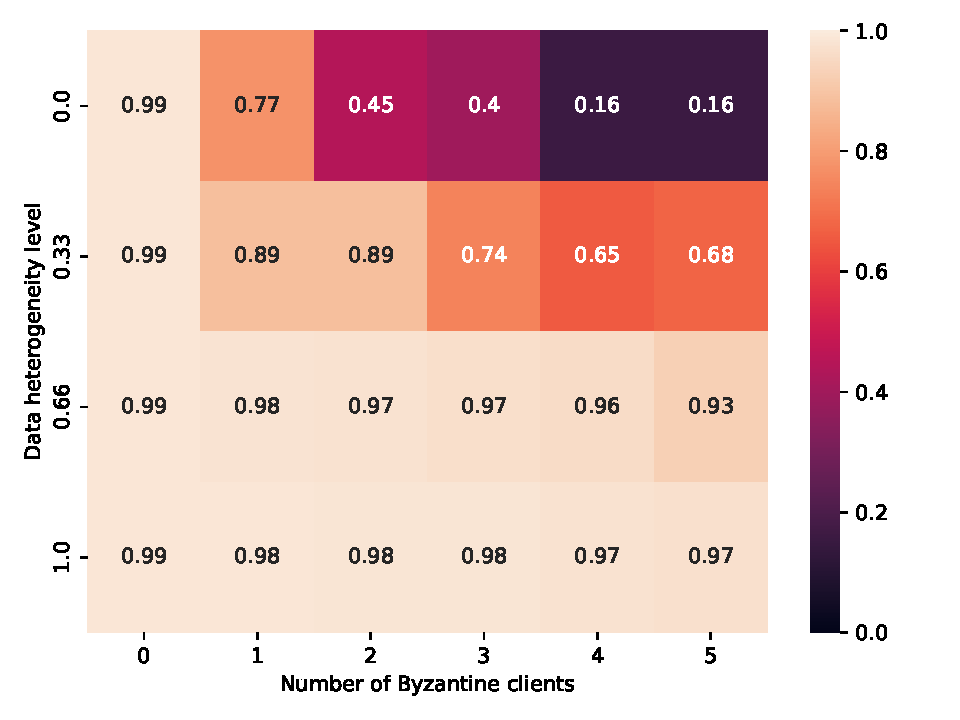
\includegraphics[width=\textwidth]{../plots/cnn_clipped_heatmaps/best_test_mnist_cnn_mnist_gamma_similarity_niid_NNM_ARC_nb_honest_clients_10_tolerated_f_equal_real.pdf}
        \caption{Best Overall (Worst-Case)}
    \end{subfigure}
    \hfill
    \begin{subfigure}[b]{0.48\textwidth}
        \centering
        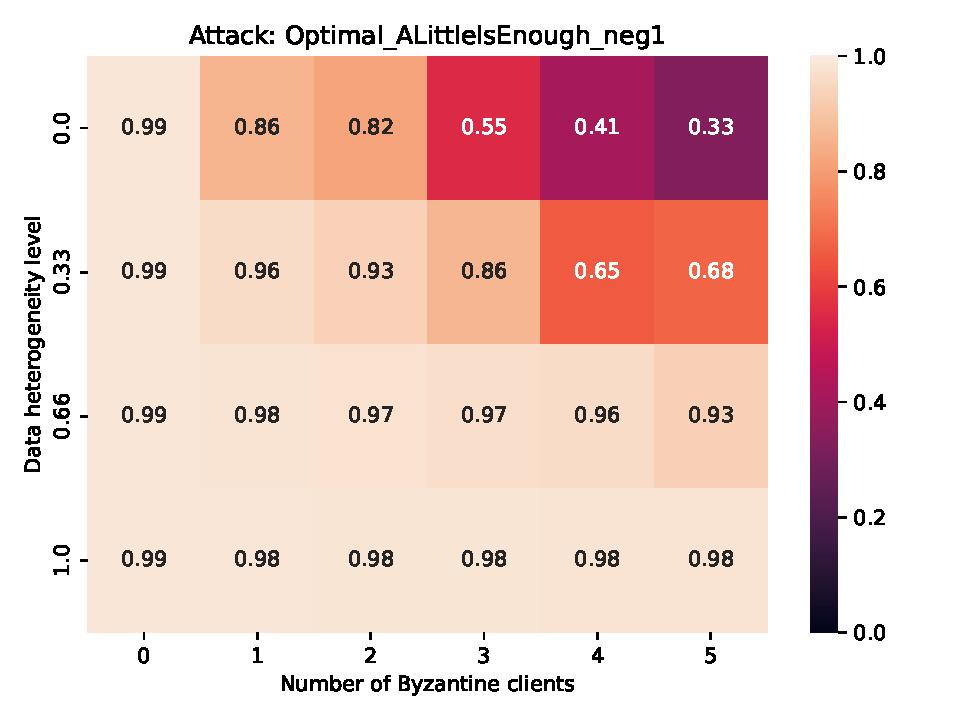
\includegraphics[width=\textwidth]{../plots/cnn_clipped_heatmaps/best_test_Optimal_ALittleIsEnough_neg1_mnist_cnn_mnist_gamma_similarity_niid_NNM_ARC_nb_honest_clients_10_tolerated_f_equal_real.pdf}
        \caption{Best under OptALIE}
    \end{subfigure}
    
    \vspace{0.2cm}
    \begin{subfigure}[b]{0.48\textwidth}
        \centering
        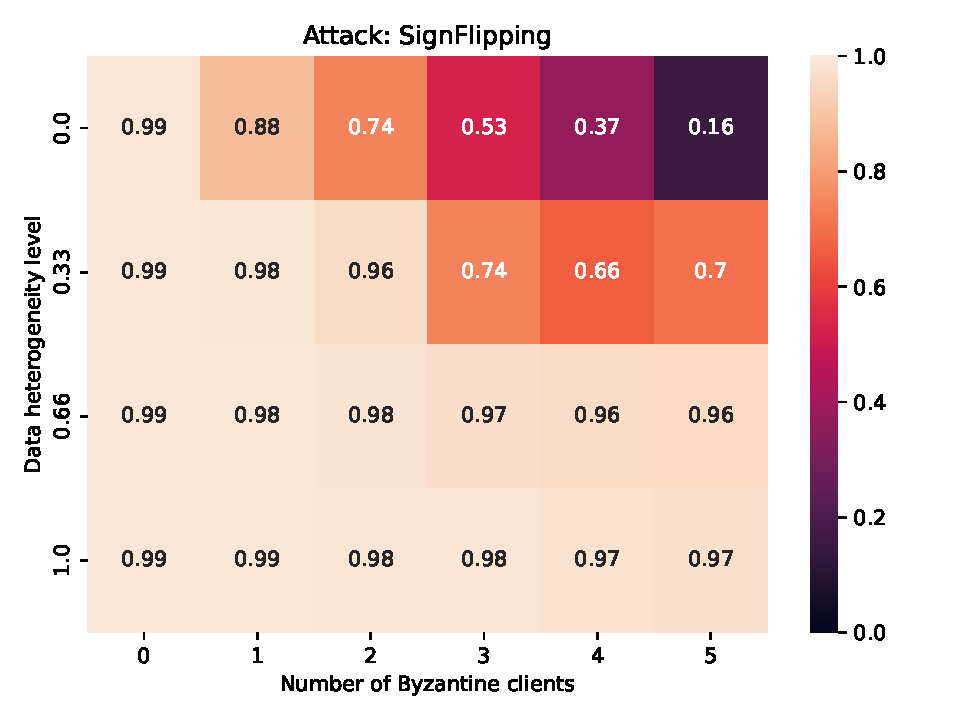
\includegraphics[width=\textwidth]{../plots/cnn_clipped_heatmaps/best_test_SignFlipping_mnist_cnn_mnist_gamma_similarity_niid_NNM_ARC_nb_honest_clients_10_tolerated_f_equal_real.pdf}
        \caption{Best under Sign Flipping}
    \end{subfigure}
    \hfill
    \begin{subfigure}[b]{0.48\textwidth}
        \centering
        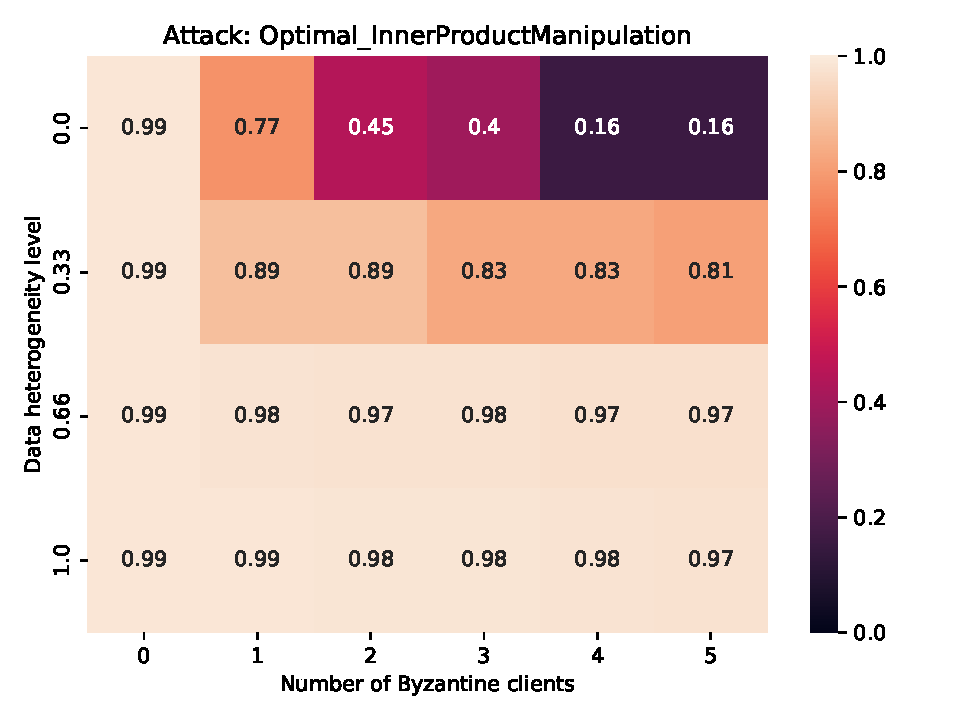
\includegraphics[width=\textwidth]{../plots/cnn_clipped_heatmaps/best_test_Optimal_InnerProductManipulation_mnist_cnn_mnist_gamma_similarity_niid_NNM_ARC_nb_honest_clients_10_tolerated_f_equal_real.pdf}
        \caption{Best under OptIPM}
    \end{subfigure}
    \caption{Robustness heatmaps for CNN with manual Gradient Clipping.}
\end{figure}

\clearpage
\section{Gradient Analysis: Clip vs. No Clip}
These plots compare the gradient norms and deviation metrics between clipped and non-clipped networks.

\begin{figure}[htbp]
    \centering
    \begin{subfigure}[b]{0.48\textwidth}
        \centering
        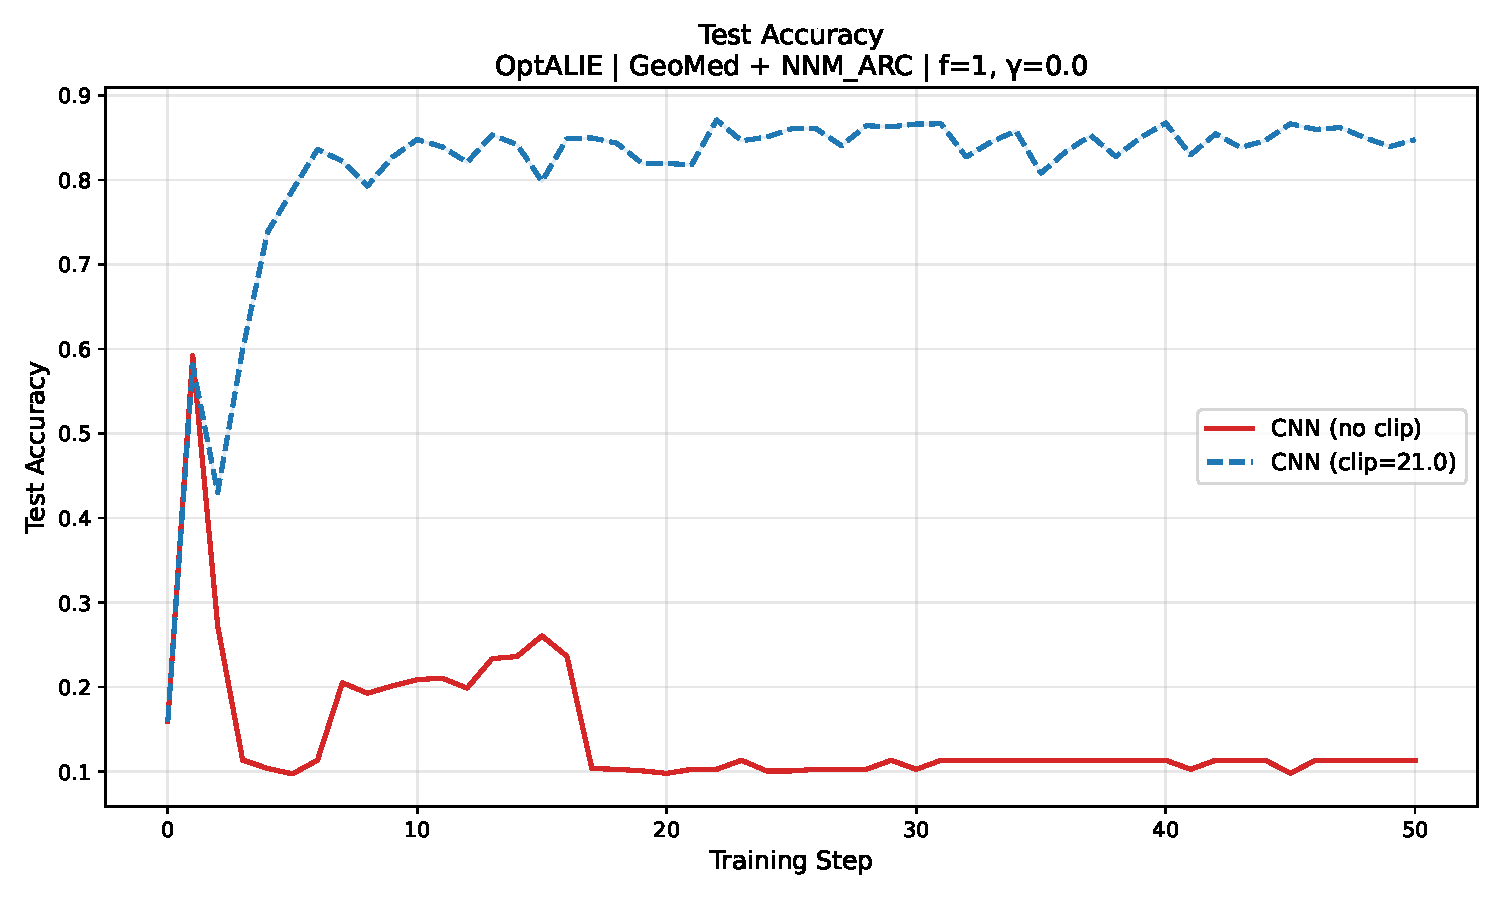
\includegraphics[width=\textwidth]{../plots/clip_vs_noclip/test_accuracy_OptALIE.pdf}
        \caption{Test Accuracy (OptALIE)}
    \end{subfigure}
    \hfill
    \begin{subfigure}[b]{0.48\textwidth}
        \centering
        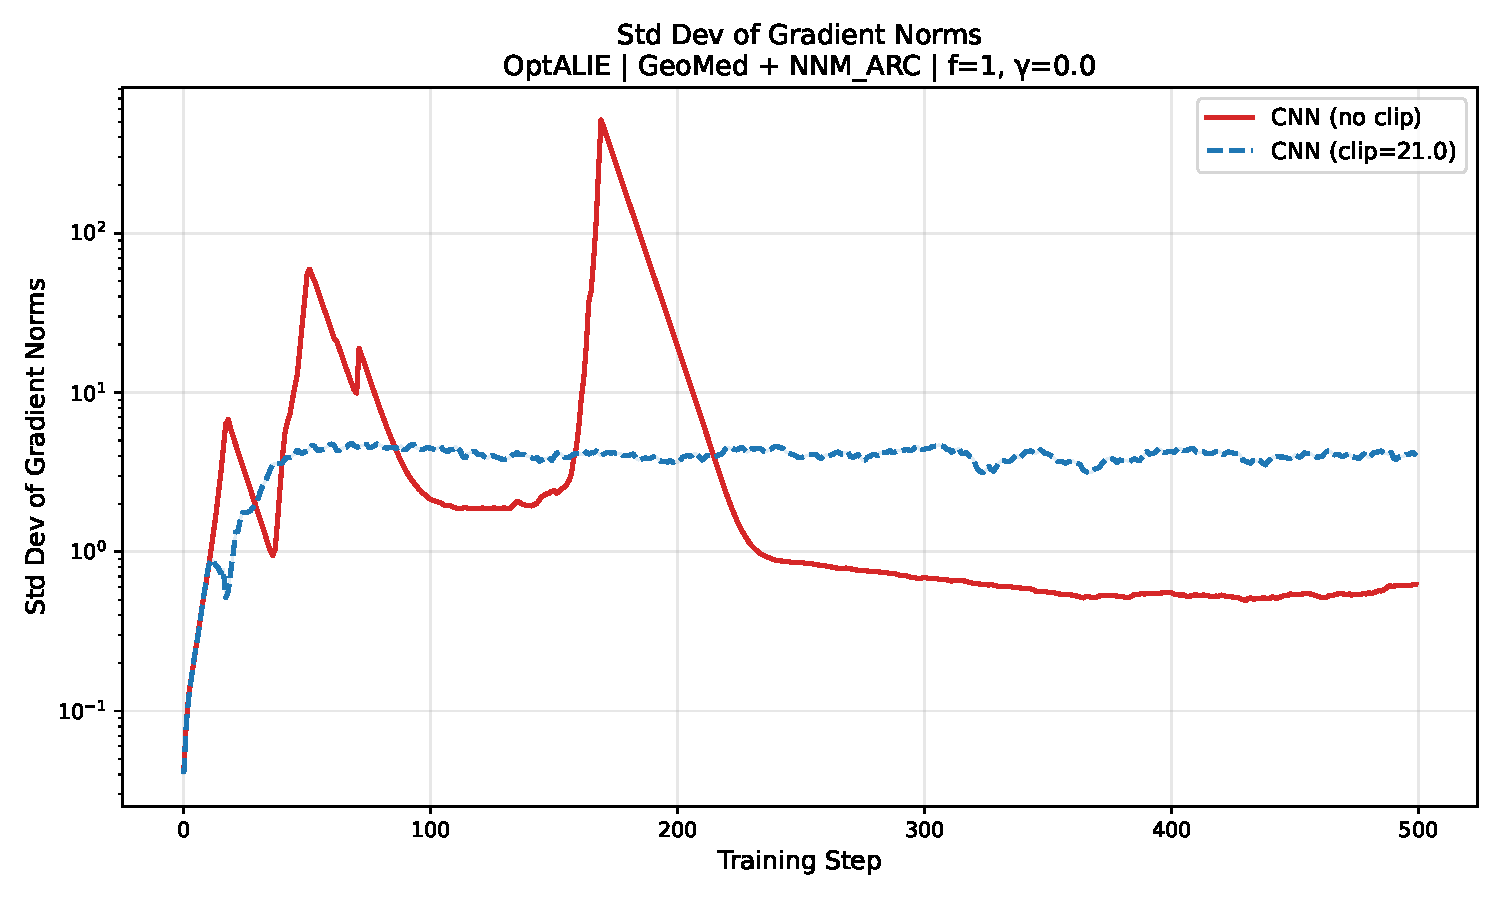
\includegraphics[width=\textwidth]{../plots/clip_vs_noclip/honest_grad_norm_std_OptALIE.pdf}
        \caption{Grad Norm Std (OptALIE)}
    \end{subfigure}

    \vspace{0.2cm}
    \begin{subfigure}[b]{0.48\textwidth}
        \centering
        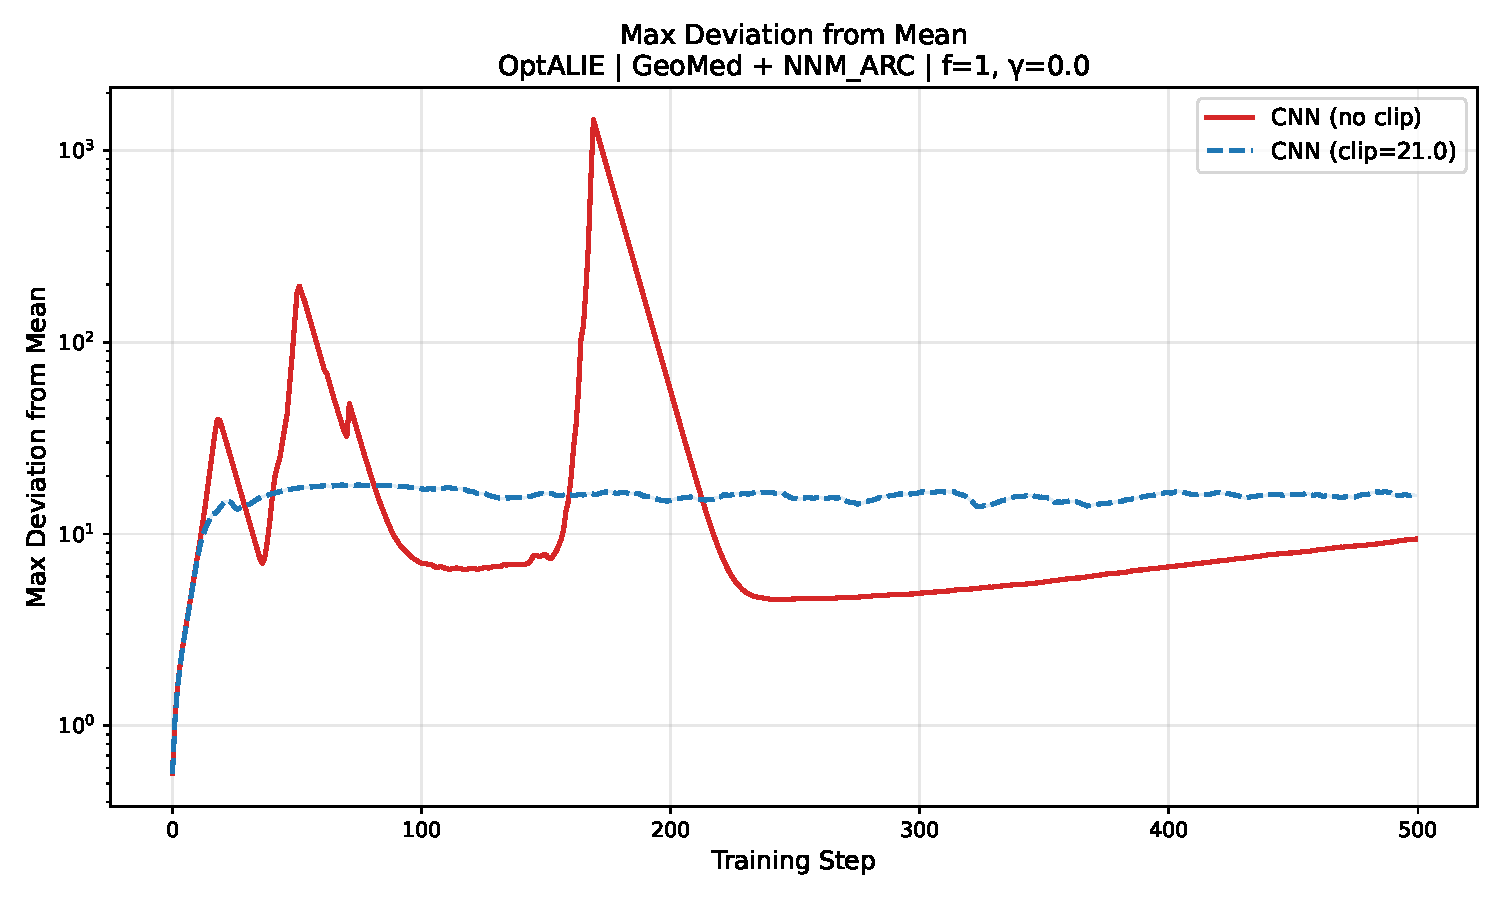
\includegraphics[width=\textwidth]{../plots/clip_vs_noclip/honest_max_deviation_OptALIE.pdf}
        \caption{Max Deviation (OptALIE)}
    \end{subfigure}
    \hfill
    \begin{subfigure}[b]{0.48\textwidth}
        \centering
        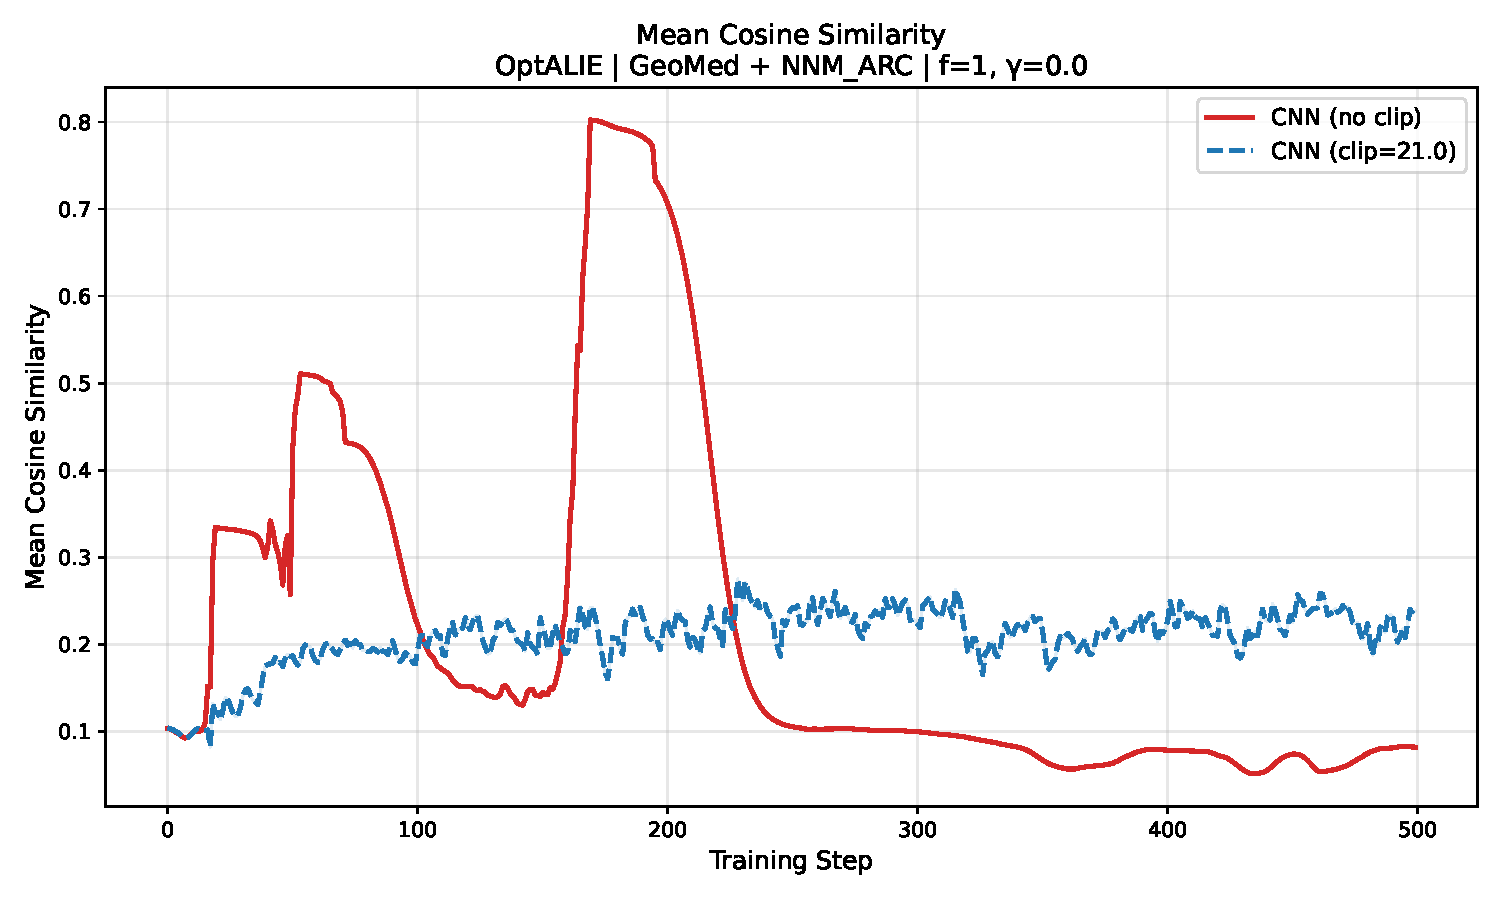
\includegraphics[width=\textwidth]{../plots/clip_vs_noclip/honest_mean_cos_sim_OptALIE.pdf}
        \caption{Mean Cosine Sim (OptALIE)}
    \end{subfigure}
    \caption{Clip vs NoClip dynamics under OptALIE.}
\end{figure}

\clearpage
\section{Activation Ablation (Tanh vs. ReLU)}
These plots compare different activation functions (e.g., Tanh which naturally saturates vs. standard ReLU).

\begin{figure}[htbp]
    \centering
    \begin{subfigure}[b]{0.48\textwidth}
        \centering
        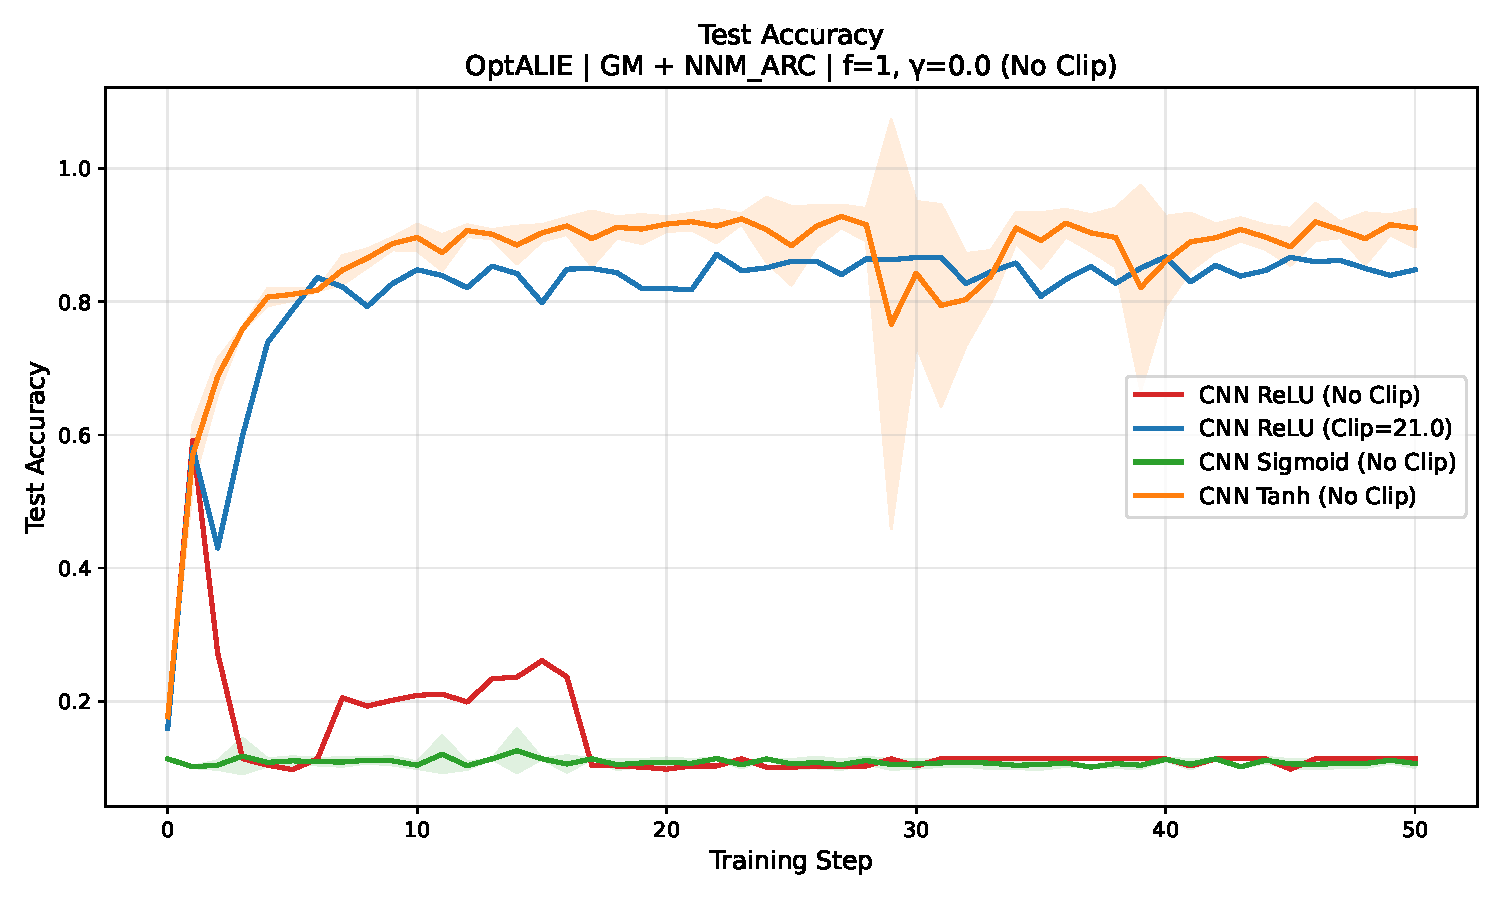
\includegraphics[width=\textwidth]{../plots/activation_ablation/test_accuracy_OptALIE.pdf}
        \caption{Test Accuracy (OptALIE)}
    \end{subfigure}
    \hfill
    \begin{subfigure}[b]{0.48\textwidth}
        \centering
        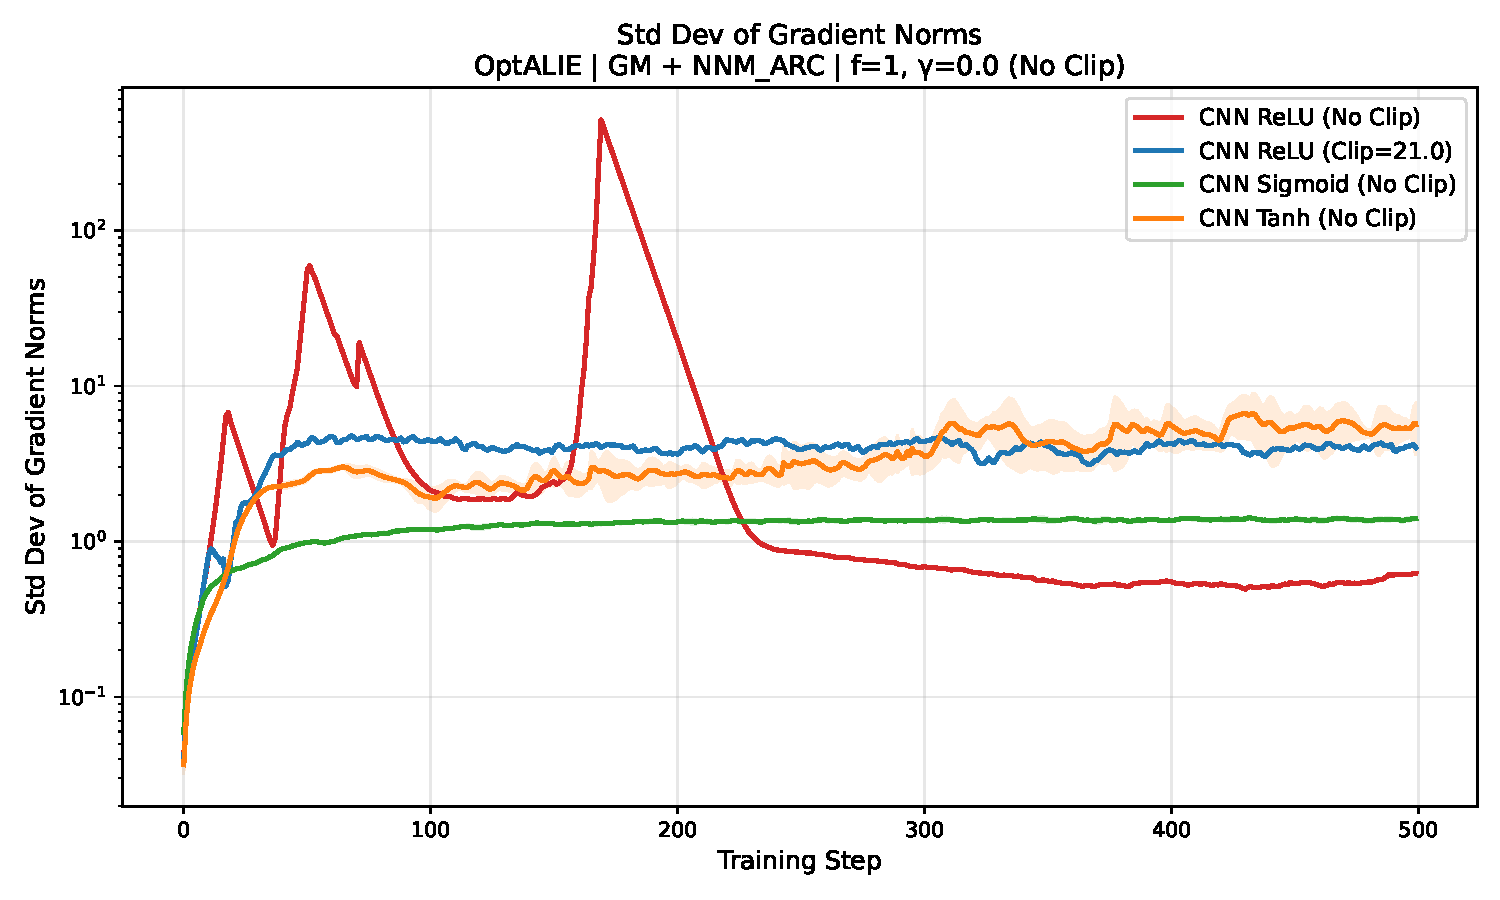
\includegraphics[width=\textwidth]{../plots/activation_ablation/honest_grad_norm_std_OptALIE.pdf}
        \caption{Grad Norm Std (OptALIE)}
    \end{subfigure}

    \vspace{0.2cm}
    \begin{subfigure}[b]{0.48\textwidth}
        \centering
        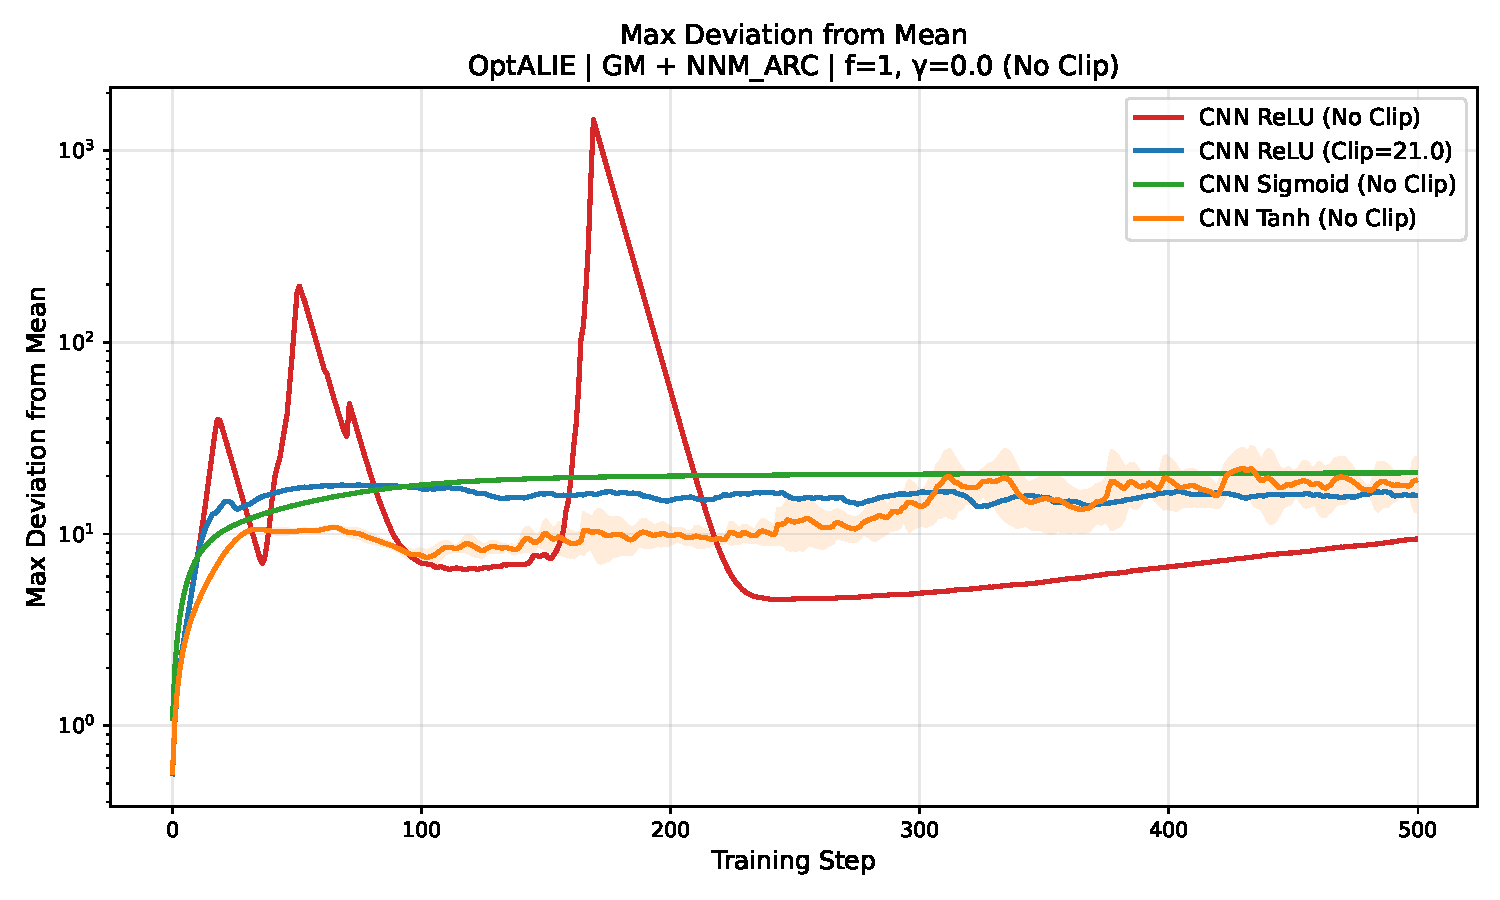
\includegraphics[width=\textwidth]{../plots/activation_ablation/honest_max_deviation_OptALIE.pdf}
        \caption{Max Deviation (OptALIE)}
    \end{subfigure}
    \hfill
    \begin{subfigure}[b]{0.48\textwidth}
        \centering
        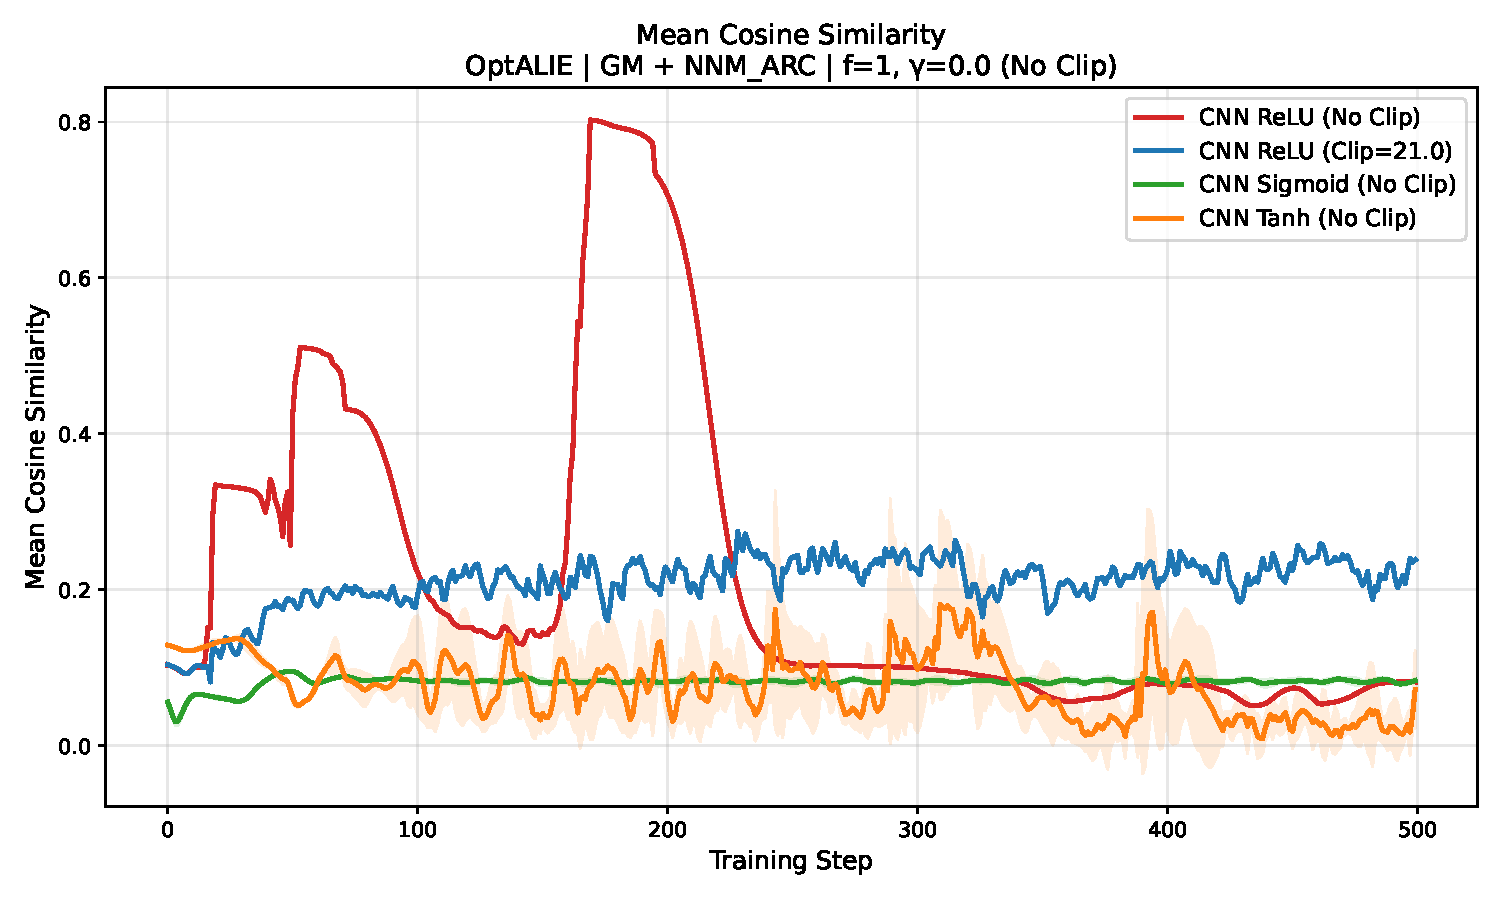
\includegraphics[width=\textwidth]{../plots/activation_ablation/honest_mean_cos_sim_OptALIE.pdf}
        \caption{Mean Cosine Sim (OptALIE)}
    \end{subfigure}
    \caption{Activation Ablation dynamics under OptALIE.}
\end{figure}

\end{document}
